\documentclass[12pt, titlepage]{article}

\usepackage{fullpage}
\usepackage[round]{natbib}
\usepackage{multirow}
\usepackage{booktabs}
\usepackage{tabularx}
\usepackage{graphicx}
\usepackage{float}
\usepackage{hyperref}
\hypersetup{
    colorlinks,
    citecolor=black,
    filecolor=black,
    linkcolor=red,
    urlcolor=blue
}
\usepackage[round]{natbib}

\newcounter{acnum}
\newcommand{\actheacnum}{AC\theacnum}
\newcommand{\acref}[1]{AC\ref{#1}}

\newcounter{ucnum}
\newcommand{\uctheucnum}{UC\theucnum}
\newcommand{\uref}[1]{UC\ref{#1}}

\newcounter{mnum}
\newcommand{\mthemnum}{M\themnum}
\newcommand{\mref}[1]{M\ref{#1}}

\title{SE 3XA3: Module Guide\\Return of the Bomberman}

\author{Team \#18, REM
		\\ Miles Jackson  jacksa7
		\\ Eitan Yehuda  yehudae
		\\ Ridhwan Chowdhury chowdr11
}

\date{\today}

\begin{document}

\maketitle

\pagenumbering{roman}
\tableofcontents
\listoftables
\listoffigures

\begin{table}[bp]
\caption{\bf Revision History}
\begin{tabularx}{\textwidth}{p{3cm}p{2cm}X}
\toprule {\bf Date} & {\bf Version} & {\bf Notes}\\
\midrule
Date 1 & 1.0 & Notes\\
Date 2 & 1.1 & Notes\\
\bottomrule
\end{tabularx}
\end{table}

\newpage

\pagenumbering{arabic}

\section{Introduction}

Return of the Bomberman is a game designed off of the original Bomber game for the SNES. This project took a simplistic and minimized version of the game and are modifying it to become a fun an interactive game that can be played by multiple players on a web browser. This document is used to show the relations between the SRS document and the implementation. Inside it will outline how and where the requirements are implemented in the code of the game. 

\section{Anticipated and Unlikely Changes} \label{SecChange}

This section lists possible changes to the system. According to the likeliness
of the change, the possible changes are classified into two
categories. Anticipated changes are listed in Section \ref{SecAchange}, and
unlikely changes are listed in Section \ref{SecUchange}.

\subsection{Anticipated Changes} \label{SecAchange}

Anticipated changes are the source of the information that is to be hidden
inside the modules. Ideally, changing one of the anticipated changes will only
require changing the one module that hides the associated decision. The approach
adapted here is called design for
change.

\begin{description}
\item[\refstepcounter{acnum} \actheacnum \label{acInput}:] The different number of characters a player can choose from.
\item[\refstepcounter{acnum} \actheacnum \label{acInput}:] The different type and number of power-ups players can use.

\end{description}

\subsection{Unlikely Changes} \label{SecUchange}

The module design should be as general as possible. However, a general system is
more complex. Sometimes this complexity is not necessary. Fixing some design
decisions at the system architecture stage can simplify the software design. If
these decision should later need to be changed, then many parts of the design
will potentially need to be modified. Hence, it is not intended that these
decisions will be changed.

\begin{description}
\item[\refstepcounter{ucnum} \uctheucnum \label{ucIO}:] 
Currently, the input solely comes from the keys on a keyboard. The keys allow the user to move their player and drop bombs. If this source of input were to change, the entire design of the game would need to be changed.  

\end{description}

\section{Module Hierarchy} \label{SecMH}

This section provides an overview of the module design. Modules are summarized
in a hierarchy decomposed by secrets in Table \ref{TblMH}. The modules listed
below, which are leaves in the hierarchy tree, are the modules that will
actually be implemented.

\begin{description}
\item [\refstepcounter{mnum} \mthemnum \label{mS}:] Server
\item [\refstepcounter{mnum} \mthemnum \label{mC}:] Client
\item [\refstepcounter{mnum} \mthemnum \label{mGL}:] GameLoop
\item [\refstepcounter{mnum} \mthemnum \label{mB}:] Bomb
\item [\refstepcounter{mnum} \mthemnum \label{mP}:] Player
\item [\refstepcounter{mnum} \mthemnum \label{mE}:] Explosion
\item [\refstepcounter{mnum} \mthemnum \label{mPU}:] PowerUp
\item [\refstepcounter{mnum} \mthemnum \label{mSG}:] StartGame
\item [\refstepcounter{mnum} \mthemnum \label{mEG}:] EndGame
\item [\refstepcounter{mnum} \mthemnum \label{mM}:] Movement
\item [\refstepcounter{mnum} \mthemnum \label{mPB}:] PlaceBomb
\item [\refstepcounter{mnum} \mthemnum \label{mCol}:] Collisions
\item [\refstepcounter{mnum} \mthemnum \label{mGenL}:] GenerateLevel

\end{description}


\begin{table}[h!]
\centering
\begin{tabular}{p{0.3\textwidth} p{0.6\textwidth}}
\toprule
\textbf{Level 1} & \textbf{Level 2}\\
\midrule

{Hardware-Hiding Module} & Server \\ & Client\\ & GameLoop\\
\midrule

\multirow{7}{0.3\textwidth}{Behaviour-Hiding Module} & Player\\
& Bomb\\
& Explosion\\
& PowerUp\\

\midrule

\multirow{3}{0.3\textwidth}{Software Decision Module} & StartGame\\
& EndGame\\
& Movement\\
& PlaceBomb\\
& Collisions\\
& GenerateLevel\\
\bottomrule

\end{tabular}
\caption{Module Hierarchy}
\label{TblMH}
\end{table}

\section{Connection Between Requirements and Design} \label{SecConnection}

The design of the system is intended to satisfy the requirements developed in
the \href{https://gitlab.cas.mcmaster.ca/chowdr11/3xa3/-/blob/master/BlankProjectTemplate/Doc/SRS/SRS.pdf}
{\textbf{SRS}}. In this stage, the system is decomposed into modules. The connection
between requirements and modules is listed in Table \ref{TblRT}.

\section{Module Decomposition} \label{SecMD}

Modules are decomposed according to the principle of ``information hiding''
proposed by \textit{ParnasEtAl1984}. The \emph{Secrets} field in a module
decomposition is a brief statement of the design decision hidden by the
module. The \emph{Services} field specifies \emph{what} the module will do
without documenting \emph{how} to do it. For each module, a suggestion for the
implementing software is given under the \emph{Implemented By} title. If the
entry is \emph{OS}, this means that the module is provided by the operating
system or by standard programming language libraries.  Also indicate if the
module will be implemented specifically for the software.

Only the leaf modules in the
hierarchy have to be implemented. If a dash (\emph{--}) is shown, this means
that the module is not a leaf and will not have to be implemented. Whether or
not this module is implemented depends on the programming language
selected.

\subsection{Hardware Hiding Modules ()}

\begin{description}
\item[Secrets:]The data structure and algorithm used to implement the virtual input and output
  hardware from the user's keyboard.
\item[Services:]Serves as a virtual hardware used by the rest of the
  system. This module provides the interface between the hardware and the
  software. So, the system can use it to display outputs or to accept inputs.
\item[Implemented By:] Operating System
\end{description}

\subsubsection{Server Module (\mref{mS})}

\begin{description}
\item[Secrets:] Contains server port and other information about the server.
\item[Services:] Creates server to play on and and echos input signals from one player to all of the players in the game.
\item[Implemented By:] Return of the Bomberman
\end{description}

\subsubsection{Client Module (\mref{mC})}

\begin{description}
\item[Secrets:] Contains responses to signals received from the server.
\item[Services:] Sends input signals to the server as well as receiving signals from other players. 
\item[Implemented By:] Return of the Bomberman
\end{description}

\subsubsection{GameLoop Module (\mref{mGL})}

\begin{description}
\item[Secrets:] Contains details about the current state of the game.
\item[Services:] Acts as a controller for the game recognizing events that take place and displays them in the game.
\item[Implemented By:] Return of the Bomberman
\end{description}


\subsection{Behaviour-Hiding Module}

\begin{description}
\item[Secrets:]The contents of the required behaviours.
\item[Services:]Includes programs that provide externally visible behaviour of
  the system as specified in the software requirements specification (SRS)
  documents. This module serves as a communication layer between the
  hardware-hiding module and the software decision module. The programs in this
  module will need to change if there are changes in the SRS.
\item[Implemented By:] Return of the Bomberman
\end{description}

\subsubsection{Bomb Module (\mref{mB})}

\begin{description}
\item[Secrets:]Contains the position, radius and time for detonation of the bomb.
\item[Services:]Can be called to generate bomb object on board and calls explosion.
\item[Implemented By:] Return of the Bomberman
\end{description}

\subsubsection{Player Module (\mref{mP})}

\begin{description}
\item[Secrets:] Contains information on a player including location and ID.
\item[Services:] Provides a playable character than can be controlled by a user with the help of other modules.
\item[Implemented By:] Return of the Bomberman
\end{description}

\subsubsection{Explosion Module (\mref{mE})}

\begin{description}
\item[Secrets:] Contains radius, animation and central position of an Explosion.
\item[Services:] Provides an explosion which can interact with other objects in the game. 
\item[Implemented By:] Return of the Bomberman
\end{description}

\subsubsection{PowerUp Module (\mref{mPU})}

\begin{description}
\item[Secrets:] Contains the position and type of power-up.
\item[Services:] Provides a power-up that can be spawned when a soft wall is destroyed.
\item[Implemented By:] Return of the Bomberman 
\end{description}

\subsubsection{StartGame Module (\mref{mSG})}

\begin{description}
\item[Secrets:]The signal received to start the game.
\item[Services:]Calls Generate Level and starts the game loop.
\item[Implemented By:] Return of the Bomberman
\end{description}

\subsubsection{EndGame Module (\mref{mEG})}

\begin{description}
\item[Secrets:]The conditions required for game to be over.
\item[Services:]Determines when game is over and stops game loop.
\item[Implemented By:] Return of the Bomberman
\end{description}



\subsubsection{PlaceBomb Module (\mref{mPB})}

\begin{description}
\item[Secrets:]The location and radius of a bomb to be placed.
\item[Services:] Provides a function to be called to place a bomb when a place bomb signal is received from the server.
\item[Implemented By:] Return of the Bomberman
\end{description}


\subsection{Software Decision Module}

\begin{description}
\item[Secrets:] The design decision based on mathematical theorems, physical
  facts, or programming considerations. The secrets of this module are
  \emph{not} described in the SRS.
\item[Services:] Includes data structure and algorithms used in the system that
  do not provide direct interaction with the user. 
  % Changes in these modules are more likely to be motivated by a desire to
  % improve performance than by externally imposed changes.
\item[Implemented By:] Return of the Bomberman
\end{description}

\subsubsection{Movement Module (\mref{mM})}

\begin{description}
\item[Secrets:]The current location of the player on the board and the current board state.
\item[Services:]Enables player movement. Checks player collisions with walls and ensures player does not move through walls.
\item[Implemented By:] Return of the Bomberman
\end{description}

\subsubsection{Collisions Module (\mref{mCol})}

\begin{description}
\item[Secrets:] Contains conditions on which a player has deemed to have collided with a Explosion. 
\item[Services:] Provides a function to check if a play has collided with a Explosion and kills the player if ther did.
\item[Implemented By:] Return of the Bomberman
\end{description}

\subsubsection{GenerateLevel Module (\mref{mGenL})}

\begin{description}
\item[Secrets:] Contains the template for the game and means to create a fresh game board.
\item[Services:] Randomly generates the level to be played filling it with players, soft/hard walls and power-ups.
\item[Implemented By:] Return of the Bomberman
\end{description}



\section{Traceability Matrix} \label{SecTM}

This section shows two traceability matrices: between the modules and the
requirements and between the modules and the anticipated changes.

% the table should use mref, the requirements should be named, use something
% like fref
\begin{table}[H]
\centering
\begin{tabular}{p{0.2\textwidth} p{0.6\textwidth}}
\toprule
\textbf{Req.} & \textbf{Modules}\\
\midrule
FR1 & \mref{mS}, \mref{mC}, \mref{mGL}, \mref{mM}\\
FR2 & \mref{mS}, \mref{mC}, \mref{mGL}, \mref{mM}\\
FR3 & \mref{mS}, \mref{mC}, \mref{mGL}, \mref{mM}\\
FR4 & \mref{mS}, \mref{mC}, \mref{mGL}, \mref{mM}\\
FR5 & \mref{mS}, \mref{mC}, \mref{mGL}, \mref{mB}, \mref{mPB}\\
FR6 & \mref{mGL}, \mref{mPU}, \mref{mP}, \mref{mB}\\
FR7 & \mref{mGL}, \mref{mB}, \mref{mE}\\
FR8 & \mref{mGL}, \mref{mB}, \mref{mP}, \mref{mPU}, \mref{mPB}\\
FR9 & \mref{mGL}, \mref{mB}, \mref{mPB}\\
FR10 & \mref{mGL}, \mref{mB}, \mref{mE}, \mref{mCol}\\
FR11 & \mref{mGL}, \mref{mB}, \mref{mE}, \mref{mCol}\\
FR12 & \mref{mGL}, \mref{mP}, \mref{mCol}\\
FR13 & \mref{mGL}, \mref{mP}, \mref{mB}, \mref{mE}, \mref{mCol}\\
FR14 & \mref{mGL}, \mref{mP}, \mref{mEG}\\
FR15 & \mref{mS}, \mref{mC}, \mref{mGL}, \mref{mP}, \mref{mEG}\\
FR16 & \mref{mS}, \mref{mC}, \mref{mGL}, \mref{mP}, \mref{mEG}\\
\bottomrule
\end{tabular}
\caption{Trace Between Requirements and Modules}
\label{TblRT}
\end{table}

\begin{table}[H]
\centering
\begin{tabular}{p{0.2\textwidth} p{0.6\textwidth}}
\toprule
\textbf{AC} & \textbf{Modules}\\
\midrule
\acref{acHardware} & \mref{mP}\\
\acref{acInput} & \mref{mPU}\\
\bottomrule
\end{tabular}
\caption{Trace Between Anticipated Changes and Modules}
\label{TblACT}
\end{table}

\section{Use Hierarchy Between Modules} \label{SecUse}

In this section, the uses hierarchy between modules is
provided. \textit{Parnas1978} said of two programs A and B that A {\em uses} B if
correct execution of B may be necessary for A to complete the task described in
its specification. That is, A {\em uses} B if there exist situations in which
the correct functioning of A depends upon the availability of a correct
implementation of B.  Figure \ref{FigUH} illustrates the use relation between
the modules. It can be seen that the graph is a directed acyclic graph
(DAG). Each level of the hierarchy offers a testable and usable subset of the
system, and modules in the higher level of the hierarchy are essentially simpler
because they use modules from the lower levels.

\begin{figure}[H]
\centering
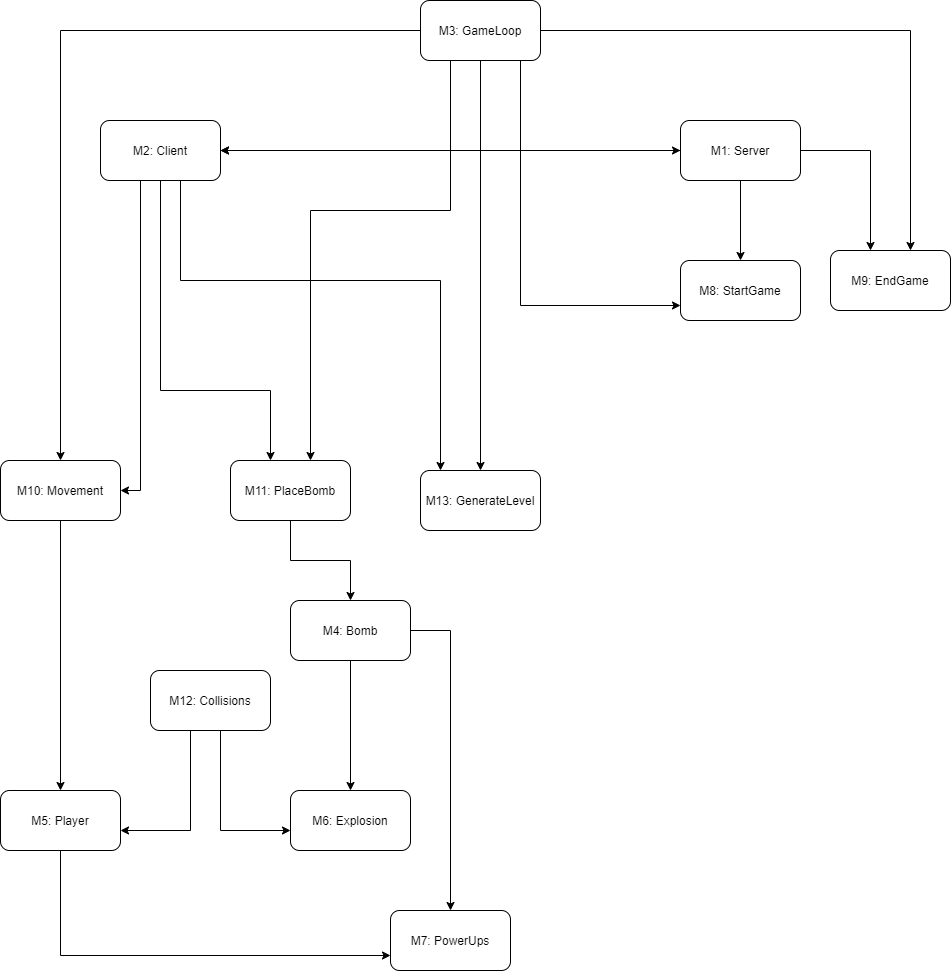
\includegraphics[width=0.7\textwidth]{UsesHierarchy.png}
\caption{Use hierarchy among modules}
\label{FigUH}
\end{figure}

%\section*{References}

\bibliographystyle {plainnat}
\bibliography {MG}

\end{document}